\chapter{Introdução}

De antemão, gostaria de dizer que sou um Trooper apaixonado e advogo sempre em causa da Hotmart em todos os lugares que vou, quer seja falando bem da empresa, quer seja incentivando meus amigos a participarem como produtores ou como Troopers. Por isso, tomo a liberdade de tecer algumas críticas construtivas sempre prezando pelo crescimento da empresa.

Como é de conhecimento geral, a Hotmart é um excelente lugar para se conviver, contar histórias, dividir momentos, criar novas soluções e fazer novas amizades. Porém, não podemos dizer o mesmo sobre o nosso ambiente de trabalho. Eu entendo que o ambiente de trabalho não é somente aquele onde vc convive, mas aquele onde você executa as ações que caracterizam seu trabalho da forma como deveria ser.

Eu, como desenvolvedor, não posso afirmar que me sinto completamente seguro ou à vontade em meu local de trabalho. Afinal de contas, há regras de negócio estão espalhadas por diversos trechos de código ou na mente da quem desenvolveu, tenho que revisar códigos que nem sei muito bem do que se trata, sou obrigado a colocar qualidade em algo onde não há referência de qualidade, recebo mais 100 emails de alertas diariamente em minha caixa de email, quando estou de plantão, tenho que lidar com projetos os quais conheço pouco ou quase nada, e assim por diante, tenho que parar meu trabalho frequentemente para atender tickets iu reuniões que não são do meu interesse. 

Eis os fatos:
\begin{enumerate}
    \item As lideranças entendam que mudar o \emph{core business} é delicado ou dão pouca importância para isso
    \item Muitos Troopers compartilham dessa insatisfação mas são discrentes de que mudanças vão acontecer
    \item Este processo complicado e confuso faz parte da história da maioria das empresas
\end{enumerate}

\section{Em time que está ganhando não se mexe, será?}
Como dizia minha professora Mirella Moro: 
\begin{quote}
A diferença entre hardware e software é: hardware você chuta e software você xinga.
\end{quote}



% Falar sobre que softeare mao eh visro
% colocar aqui o exemplo de se fazer uma

\section{O Monte Everest}

\section{Conquistando a Maturidade}

Toda empresa ou indivíduo quando que nasce, passa pelo processo do seu descobrimento profissional ou individual onde toma escolhas acreditando estar indo na direção correta. Muitas dessas escolhas, em um primeiro momento, podem parecer boas decisões. Outras porém, podem se revelar escolhas ruins. O fato é que não é possível perceber quais são as boas e as más decisões. Algumas delas, por piores que sejam, pelo menos ajudam a chegar em algum caminho. Assim que atingimos esse caminho, conseguimos acertar mais do que errar, ou a amplitude de nossas ações diminui drasticamente e as coisas vão se moldando de uma uma forma mais sólida do que antes. Este fenômeno é conhecido como maturidade.

\begin{figure}[H]
    \centering
    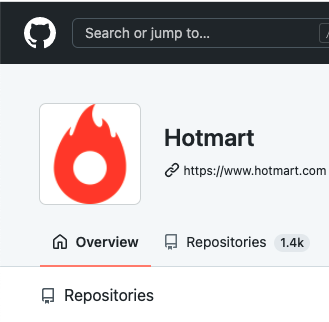
\includegraphics[scale=0.60,keepaspectratio=true]{images/01.png}
    \caption{Processo de amadurecimento}
    \label{mature_process}
\end{figure}

Como indivíduo ou como empresa, não é possível voltar atrás e fazer as melhores escolhas. Mas como software, isso é possível graças a consolidação do conhecimento adquirido até o momento.

\begin{figure}[H]
    \centering
    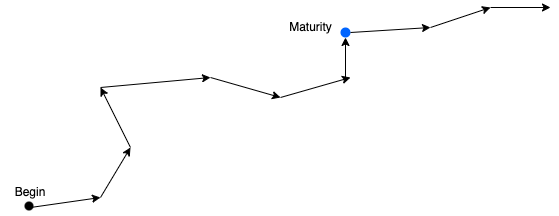
\includegraphics[scale=0.60,keepaspectratio=true]{images/02.png}
    \caption{Processo de consolidação do conhecimento}
    \label{knwledge_consolidation}
\end{figure}

Agora, mesmo que soubéssemos as melhores escolhas, de nada adiantaria chegar até aqui sem a correta manutenção de cada delas, ou seja, sendo que a cada nova decisão não fossem levadas em consideração todas as demais.

\begin{figure}[H]
    \centering
    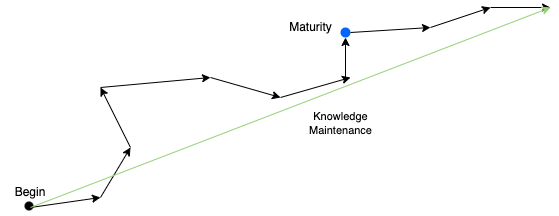
\includegraphics[scale=0.60,keepaspectratio=true]{images/03.png}
    \caption{Processo de consolidação do conhecimento}
    \label{knowledge_maintenance}
\end{figure}

